\documentclass[screen, aspectratio=43]{beamer}
\usepackage[T1]{fontenc}
\usepackage[utf8]{inputenc}

% Use the NTNU-temaet for beamer 
% \usetheme[style=ntnu|simple|vertical|horizontal, 
%     language=bm|nn|en, 
%     smalltitle, 
%     city=all|trondheim|alesund|gjovik]{ntnu2017}
\usetheme[style=ntnu,language=en]{ntnu2017}

\usepackage[english]{babel}
\usepackage[style=numeric,backend=biber,natbib=false,sorting=none]{biblatex}

\title[PCW-d1]{Physical Computing Workshop: Day 4}
\subtitle{Mini hackathon and the real world}
\author[A. Xamb{\'o}]{Anna Xamb{\'o}}
\institute[NTNU]{Department of Music, NTNU}
\date{19 October 2018}
%\date{} % To have an empty date

\addbibresource{example.bib} % Add bibliography database

% Set the reference style to numeric.
% See here: http://tex.stackexchange.com/questions/68080/beamer-bibliography-icon
\setbeamertemplate{bibliography item}[text] 

% Set bibliography fonts to a small size.
\renewcommand*{\bibfont}{\footnotesize}

\begin{document}

\begin{frame}
  \titlepage
\end{frame}
%
\begin{frame}
  \frametitle{Learning Outcomes}
  \begin{itemize}
    \item Be capable of synthesizing and being critical on self-reflective practice. 
    \item Develop peer critique practices.
    \item Be able to express a concept from ideation to prototyping.
    \item Get a sense on how to combine and build on previous code.
    \item Explore how to design a custom-made musical instrument based on performance, engineering and originality/creativity.  
    \item Learn how to present a custom-made musical instrument.
    \item Demonstrate a custom-made musical instrument in a performance setting.
    \item Reflect on the custom-made musical instrument and performance using a blogging style.
  \end{itemize}
\end{frame}
\begin{frame}
  \frametitle{Preparation: Reading}
        \begin{itemize}
        \item Read the three daily blog posts written by your group during the physical computing workshop and be ready to present it in 10 minutes.
         \end{itemize}
\end{frame}
%
\begin{frame}
  \frametitle{Preparation: What to Bring to Class?}
        \begin{itemize}
        \item All the required items at hand to develop the final prototype.
         \end{itemize}
\end{frame}
%
\begin{frame}
  \frametitle{Preparation: What We Do Provide?}
        \begin{itemize}
        \item We can provide any of the items used during the workshop under request.       
         \end{itemize}
\end{frame}
%
\begin{frame}
  \frametitle{Outline}
      \begin{itemize}
	\item Block I: Reflective recap
	\item Block II: Mini Hackathon
	\item Block III: Rehearsal and final performance
    \end{itemize}  
\end{frame}
%
\begin{frame}
  \frametitle{Reflective recap: 9:15--9:45}
  Each group is asked to summarize the week through the three blog posts during 10 min (a countdown timer will be used). 
    \begin{itemize}
    	\item 9:15--9:25 Group A
	\item 9:25--9:35 Group B
	\item 9:35--9:45 Group C
    \end{itemize}
\end{frame}
%
\begin{frame}
  \frametitle{Conceptualization: 9:45--11:15}
  The class should split into teams and define the concept of their prototype (the concept should shape the technology and not the other way around!). Some idea generation techniques include brainstorming, mindmapping, storyboarding, and so on. Here you can find some idea generation techniques: \url{https://www.cleverism.com/18-best-idea-generation-techniques/}
    \begin{itemize}
    	\item Trondheim: Due to the Open Day, two groups can stay in the portal and the third group can go to the 16-channel room.
    \end{itemize}
\end{frame}
%
\begin{frame}
  \frametitle{Presentations of the prototype concepts: 11:15--12:00}
  Each group is asked to present their prototype idea during 10 min + 5 min more for Q\&A (a countdown timer will be used).
    \begin{itemize}
    	\item 11:15--11:30 Group B
	\item 11:30--11:45 Group C
	\item 11:45--12:00 Group A
    \end{itemize}
\end{frame}
%
\begin{frame}
  \frametitle{Mini-hackathon \& rehearsal: 12:00--15:00}
  Each group has 3 hours to develop their idea and rehearse how they are going to pitch it. 
    \begin{itemize}
    	\item Trondheim: Due to the Open Day, two groups can stay in the portal and the third group can go to the 16-channel room.
	\item All: Due to the Open Day in Trondheim, groups of students will come and enquiry about what you are doing / hacking 13:00--14:00. This can be a good exercise to get feedback on the prototype.
    \end{itemize}
    {\tiny Some tips \& tricks on how to pitch a technology idea:
     \begin{itemize}
    	\item 18 Pitching Essentials: How to Pitch an Idea to Investors (and Early Customers): \url{https://www.ryrob.com/how-to-pitch/}
      \end{itemize}	
    }
\end{frame}
%
\begin{frame}
  \frametitle{Final performance: 15:00--16:00}
  Each group is asked to present their prototype idea during 15 min, where they should pitch their idea and perform with the instrument (a countdown timer will be used). We will have a special guest: one of the three jury members of the mini-hackathon will be present during the oral presentations. The other two jury members will read the blog post and listen to the audio recording of the performance to assess each music hack.
    \begin{itemize}
    	\item 15:00--15:15 Group C
	\item 15:15--15:30 Group A
	\item 15:30--15:45 Group B
	\item 15:45--15:55 Free improvisation with all the three groups
	\item 15:55--16:00 Closing
    \end{itemize}
\end{frame}
%
\begin{frame}
  \frametitle{Post-activities}
    \begin{itemize}
         \item Fill in the following questionnaire after the workshop ends (ideally before Monday, October 22, 2018, at 14:00): \\
 	\url{https://goo.gl/tUn8LJ}       
    	\item The final blog post about the music hack should be published by Monday, October 22, 2018, at 14:00. In the blog post, make sure to combine text with media to communicate the concept of your music hack, from ideation to prototype. The blog post will be sent together with the audio recording of the performance to the two jury members who are not able to come presentially to the mini-hackathon.
	\item The final grade of the workshop will be independent of the results of the mini-hackathon. The criteria of the workshop evaluation is explained in ``pcw-intro.pdf''.
    \end{itemize}
\end{frame}
%
\begin{frame}
  \frametitle{Jury members}
    \begin{itemize}
    	\item We have the privilege to have three jury members for this mini-hackathon:
	    \begin{itemize}
	    	\item \textbf{Tone Åse}, Associate Professor and Singer working with voice, improvisation and live electronics (Department of Music, NTNU, Norway): \url{https://www.ntnu.no/ansatte/tone.ase}
		\item \textbf{Charles Martin}, Postdoctoral Fellow specialising in music technology and machine learning (Department of Informatics, UiO, Norway): \url{https://www.mn.uio.no/ifi/english/people/aca/charlepm/index.html}
		\item \textbf{Gerard Roma}, Postdoctoral Fellow specialising in real-time computer music systems and sound analysis and retrieval (Department of Music, University of Huddersfield, Norway): \url{http://www.flucoma.org/}
        	    \end{itemize}
    \end{itemize}
\end{frame}
%
\begin{frame}
  \frametitle{Criteria of evaluation (jury)}
  The criteria of evaluation that the jury members will look at are the following:
    \begin{itemize}
    	\item Originality / Creativity
	\item Design / Engineering
	\item Performance / Musicality
    \end{itemize}
\end{frame}
%
\begin{frame}
  \frametitle{Prize}
  \begin{figure}
	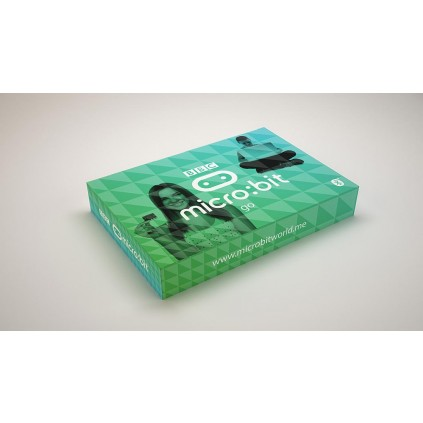
\includegraphics[scale=0.3]{img/microbit-go-main_5_1.jpg}
	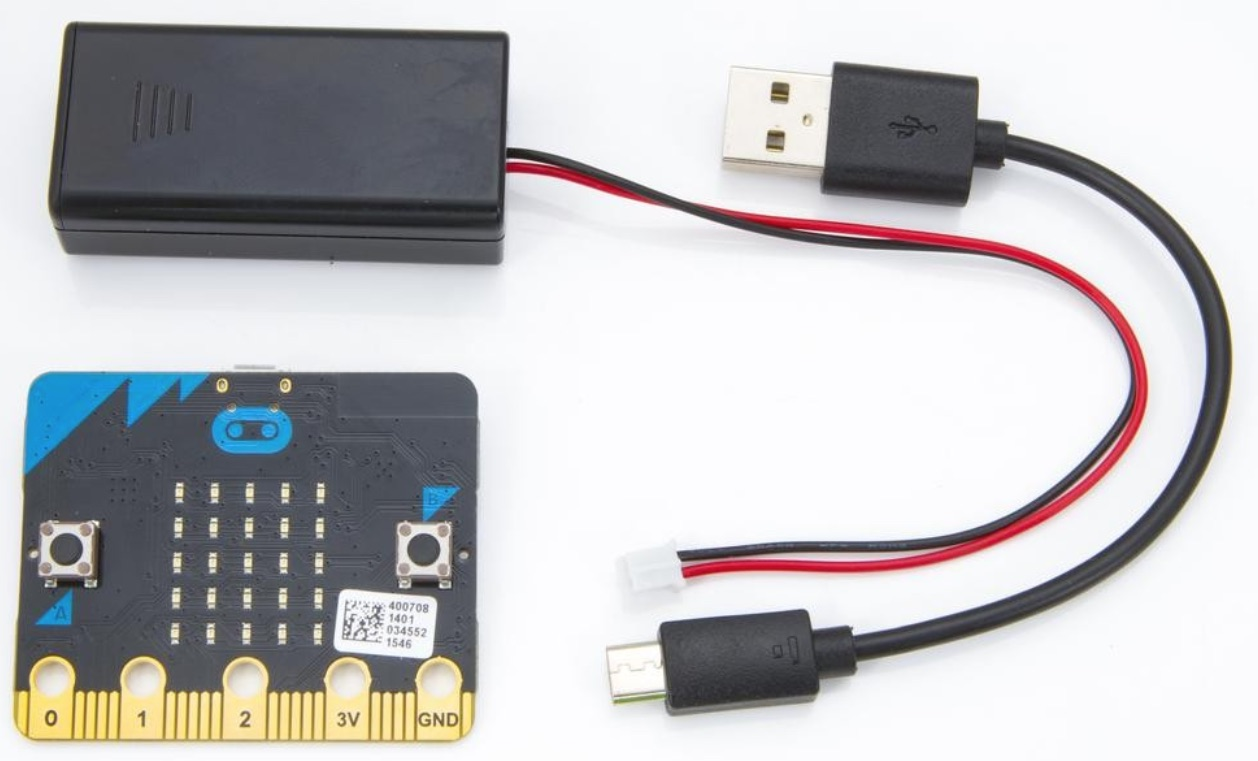
\includegraphics[scale=0.1]{img/microbit-go.jpg}
  \end{figure}
  The best music hack will be awarded with...
    \begin{itemize}
    	\item A  \textbf{BBC micro:bit Go!} for each team member!: \url{https://microbit.org/}
	\begin{itemize}
		\item Let's make some noise! It's the BBC micro:bit MusicFest: \\
		\url{https://www.microbit.co.uk/musicfest}
		\item Music — BBC micro:bit MicroPython 0.5.0 documentation:\\ 
		\url{https://microbit-micropython.readthedocs.io/en/latest/tutorials/music.html}
	\end{itemize}
    \end{itemize}
\end{frame}
%
\begin{frame}
  \frametitle{Happy Hacking!}
    \begin{figure}
	
\includegraphics[scale=0.3]{img/ethical-hacking.jpg}
    \end{figure}	
    {\tiny Image source: \url{https://www.indiatoday.in}}
\end{frame}
%

\end{document}
